\section{Introduction}

% \subsection{Personal introduction}
% \begin{itemize}
%     \item Ich + paper + yad
% \end{itemize}

\subsection{Motivation and non-goals}
We aim in this course to make a meaningful comparison between the theoretical predictions and the experimental measurement of a fully inclusive Deeply Inelastic Scattering (DIS) cross-section.
Instead of an abstract, theoretical discussion about DIS, which can be found in a standard lecture on particle physics, we're looking here to make a connection with real-life physics solving current research questions.
The main focus is be naturally on PDF, for which DIS plays a major role.
In fact, DIS was, is, and will be a very important constrain in determining Parton Distribution Functions (PDFs) - only recently, e.g.\ starting from NNPDF4.0\cite{NNPDF:2021njg}, LHC data starts to dominate in PDF fits.
Stressing the importance and relevance of PDFs for any kind of perturbative QCD (pQCD) application and to understand the inner structure of hadrons is left to the literature~\cite{Gao:2017yyd,Heinrich:2020ybq,Amoroso:2022eow}.
In turn, DIS itself can be used to answer unresolved questions about PDFs, e.g.\ whether the proton has an intrinsic charm component~\cite{NNPDF:2023tyk}.

In order to obtain a more realistic DIS treatment, we review general pQCD features and exemplify them using DIS.
In fact, fully inclusive DIS comes in very handy, since here the effects mostly appear in their simplest form and when considering hadronic collisions, e.g.\ at the LHC, the strategies are mostly the same just more involved.
We keep a phenomenological point of view with a specific focus on the numerical implementation as, eventually, we want to compare to the experimental measurements.
We refrain from giving detailed proofs in this course and point to the standard textbooks~\cite{Leader:2011gpt,Leader:1996hm,Peskin:1995ev,Halzen:1984mc,Kronfeld:2010bx} for that.
Instead, we consider different features as given and focus on their practical implications.
However, a major complication in this course is the interconnection between almost all features and while we discuss them here in turn, we highlight also how they are intertwined with each other.

In recent years (and much more so hopefully in the coming years), DIS has become a major research topic again thanks to the advent of the Electron Ion Collider (EIC)~\cite{Accardi:2012qut}.
While the planned physics program of the EIC goes far beyond standard fully inclusive DIS, this simplest case can serve as an introduction into more complicated topics.

The structure of this course follows in large parts the implementation of Yadism (Yet Another DIS module)~\cite{Candido:2024rkr,barontini_2026_18758473}, which is developed and used by the NNPDF collaboration in their PDF determinations.
The online documentation, which is available at
\begin{center}
    \url{https://yadism.readthedocs.io/} \,,
\end{center}
may serve as additional, more technical introduction into the topic.
Note that Yadism is an open-source project to which everybody can contribute.

Since DIS is a very wide field, it is worth spelling out explicitly some non-goals:
\begin{itemize}
    \item We only consider pQCD in the collinear framework here.
        However, because DIS is such a powerful experiment, which offers a clean access to the inner structure of the protons it can be studied using other frameworks as well, such as Color Glass Condensates~\cite{Bertilsson:2026vtu,Casuga:2026xxt} \textrightarrow{} ask H.~Mäntysaari or T.~Lappi
    \item We only consider fully inclusive cross-sections here (to be defined in \cref{sec:xs} and with a tiny exception to be discussed in \cref{sec:hq}).
        In particular, we do not consider any more complicated final states, such as, e.g., single jet or di-jet production~\cite{H1:2014cbm}.
    \item We only consider pQCD in the collinear framework here.
        While, Monte Carlo Event generators, such as, e.g., Pythia~\cite{Bierlich:2022pfr}, are rooted in collinear pQCD they eventually go much beyond and we do not consider their details here~\cite{Helenius:2026odp} \textrightarrow{} ask I.~Helenius.
    \item We only consider DIS here.
        In particular, we do not consider photo-production or elastic or diffractive cross sections.
        We define the necessary kinematics for the distinction below in \cref{sec:basics}.
    \item We compute the theoretical predictions here.
        So while we try to keep the connection to the experimental side close, we do not discuss any specific details about how to measure cross-sections.
\end{itemize}

\subsection{Requirements}

We need some basic knowledge from particle physics and, in particular, you need to be familiar with the Standard Model overview shown in \cref{fig:SM}.
\begin{figure}
    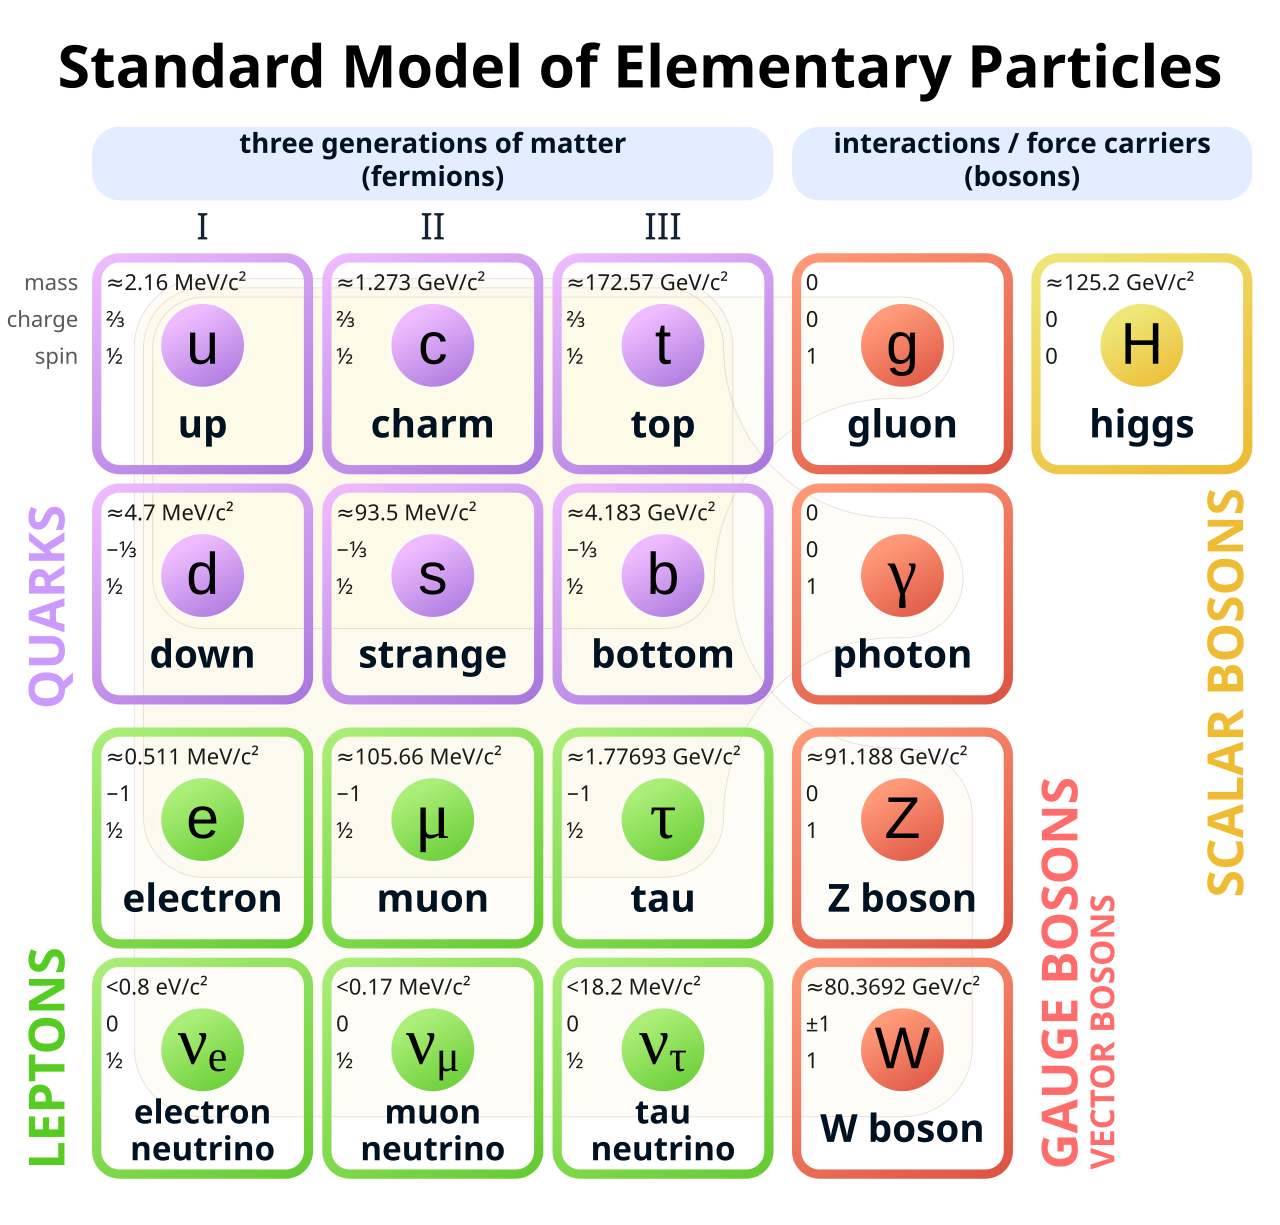
\includegraphics[width=.8\textwidth]{figures/Standard_Model_of_Elementary_Particles.svg.png}
    \caption{The Standard Model of Elementary Particles - taken from \cite{wikiSM}}
    \label{fig:SM}
\end{figure}
We discuss in this course each and everyone of these particles, with the exception of the three heaviest in each category:
the heavies quark, the top, the heaviest lepton, the tau, and the heaviest boson, the Higgs.
They work, in principle, mostly like their lighter brothers and sisters, but in practice are basically always neglected.
We give a more thorough justification to discard them when we get to the actual numbers.
All other particles explicitly appear in this course and you need to know their charges - see also \cref{fig:SM}.

\begin{tcolorbox}[title={Summary forces, particles, and charges}]
    \begin{itemize}
        \item The carrier of the strong force is the gluon
        \item Quarks have a strong charge, leptons don't
        \item The carriers of the electro-weak force are the photon, the Z boson, and the W boson
        \item Quarks and charged leptons have electro-magnetic charges
        \item Quarks and leptons have weak charges
    \end{itemize}
\end{tcolorbox}

We also need some basic knowledge from Quantum Field Theory.

\subsection{The very basics}
\label{sec:basics}
Let's start from the top:
\begin{tcolorbox}[title={DIS in words}]
    fully inclusive DIS = fully inclusive deeply inelastic scattering
\end{tcolorbox}
What does that actually mean? We begin from the back:
\begin{itemize}
    \item \enquote{scattering} means, of course, we are scattering two particles with each other.
        In this particular case, we are scattering a lepton off a hadron and to make things simple in the beginning we consider an electron is scattered off a proton.
    \item \enquote{inelastic} means we are breaking the target, the proton, apart; it shatters into many pieces.
    \item \enquote{deeply} is an adjective to inelastic and it means we are looking \enquote{deep} into the inside of the proton.
        And in order to resolve small things, as usual, we need an highly energetic probe.
    \item \enquote{fully inclusive} means we are observing a single particle in the final state, which is the electron, but nothing else.
\end{itemize}
Thus, we can write the same information again with a formula
\begin{tcolorbox}[title={DIS in formular}]
    fully inclusive DIS = $e^-(k) + p(P) \to e^-(k') + X $ with $-(k^2 - k'^2) \gg \Lambda_\text{QCD}^2$
\end{tcolorbox}
where we have assigned the four-momenta $k,P,k'$ to the incoming electron, the incoming proton and the outgoing electron respectively.




\begin{itemize}
    \item factorization theorem
    \item LO
\end{itemize}
